\documentclass{article}
% translate with >> pdflatex -shell-escape <file>

% This file is used as unit test for pgfplots, copyright by Christian Feuersaenger.
% 
% See
%   http://pgfplots.sourceforge.net/pgfplots.pdf
% for pgfplots.
%
% Any required input files (for <plot table> or <plot file> or the table package) can be downloaded
% at
% http://www.ctan.org/tex-archive/graphics/pgf/contrib/pgfplots/doc/latex/
% and
% http://www.ctan.org/tex-archive/graphics/pgf/contrib/pgfplots/doc/latex/plotdata/

\usepackage{pgfplots}
\pgfplotsset{compat=newest}

\pagestyle{empty}

\begin{document}
\pgfplotsset{every axis/.append style={cycle list={%
	red,only marks,mark options={fill=red!80!black},mark=*\\%
	black,only marks,mark options={fill=black},mark=square*\\%
	}}}
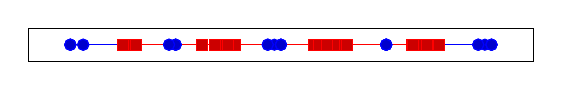
\begin{tikzpicture}
\begin{axis}[%
	width=8cm,
	height=2cm,
	xtick=\empty,
	ytick=\empty
]

\addplot plot coordinates {
	(0.968555,	0.000000)
	(0.984277,	0.000000)
	(0.030884,	0.000000)
	(0.250000,	0.000000)
	(0.750000,	0.000000)
	(0.468750,	0.000000)
	(0.750000,	0.000000)
	(0.484375,	0.000000)
	(0.968555,	0.000000)
	(0.968555,	0.000000)
	(1.000000,	0.000000)
	(1.000000,	0.000000)
	(0.030176,	0.000000)
	(0.250000,	0.000000)
	(0.250000,	0.000000)
	(0.250000,	0.000000)
	(0.750000,	0.000000)
	(1.000000,	0.000000)
	(0.500000,	0.000000)
	(0.500000,	0.000000)
	(0.234375,	0.000000)
	(0.500000,	0.000000)
	(0.750000,	0.000000)
	(0.000000,	0.000000)
	(0.750000,	0.000000)
	(0.468750,	0.000000)
	(0.500000,	0.000000)
	(0.000000,	0.000000)
	(0.468750,	0.000000)
	(0.000000,	0.000000)
	(0.750000,	0.000000)
	(0.000000,	0.000000)
	(0.234375,	0.000000)
	(1.000000,	0.000000)
};
\addplot plot coordinates {
	(0.367188,	0.000000)
	(0.625000,	0.000000)
	(0.312500,	0.000000)
	(0.656250,	0.000000)
	(0.312500,	0.000000)
	(0.148438,	0.000000)
	(0.125000,	0.000000)
	(0.640625,	0.000000)
	(0.136719,	0.000000)
	(0.875000,	0.000000)
	(0.390625,	0.000000)
	(0.828125,	0.000000)
	(0.875000,	0.000000)
	(0.656250,	0.000000)
	(0.125000,	0.000000)
	(0.343750,	0.000000)
	(0.861328,	0.000000)
	(0.312500,	0.000000)
	(0.578125,	0.000000)
	(0.578125,	0.000000)
	(0.625000,	0.000000)
	(0.375000,	0.000000)
	(0.875000,	0.000000)
	(0.812500,	0.000000)
	(0.847656,	0.000000)
	(0.589844,	0.000000)
	(0.343750,	0.000000)
	(0.125000,	0.000000)
	(0.875000,	0.000000)
	(0.125000,	0.000000)
	(0.609375,	0.000000)
	(0.156250,	0.000000)
};
\end{axis}
\end{tikzpicture}
\end{document}
